\chapter*{Úvod}
\addcontentsline{toc}{chapter}{Úvod}
% Cílem práce je navrhnout ucelený systém monitorující chod pletacích strojů ve firmě a~přizpůsobit ho co možná nejlépe potřebám firmy.

S~nápadem vytvořit systém monitorující chod pletacích strojů přišel můj děda, zakladatel firmy na výrobu ponožek.
% Jeho snem vždy bylo mít takový systém, který by částečně zastal monotónní lidskou práci a~nahradil ji efektivní automatizací.
Jeho snem vždy bylo mít systém, který by částečně zastal monotónní lidskou práci a~nahradil ji efektivní automatizací.
Tím myslel například automatické počítání vyrobených ponožek, hlášení poruch strojů a podobné monitorování výroby.

Můj systém jsem tedy navrhoval na míru pro rodinnou firmu na pletení ponožek, ve které je okolo 25 pletacích strojů. 
% Tento systém je schopen v~reálném čase zaznamenávat a~následně odesílat naměřená data ze strojů na server. 
% Pro uživatele pak systém nabízí moderní webové stránky, kde si může naměřená data přehledně zobrazit a~analyzovat.

Podle pletacích strojů, na kterých tento systém běží, jsem projekt pojmenoval Pletačka IoT. 
Systém se skládá ze tří částí.
Senzorová část, která je~připojená k~pletacímu stroji a~odesílá data.
Dále pak server, který veškerá data zpracovává a~zobrazuje je uživateli.
Poslední částí je podpůrný server, který se stará o~aktualizaci a~kontrolu správného chodu senzorů.\newline


Při~vytváření tohoto projektu jsem si dal za cíl:
\begin{itemize}
    \item projekt s~otevřeným zdrojovým kódem
    \item cenová dostupnost
    \item jednoduché přidání senzorů
    \item přehledné uživatelské rozhraní
\end{itemize}

\newpage
Pro systém jsem si stanovil tyto požadavky
\begin{itemize}
    \item Počítání upletených ponožek
    \item Zjišťování poruchovosti strojů
    \item Porovnání jednotlivých pracovních směn
    \item Monitorování průběhu výroby
\end{itemize}

\begin{figure}[htbp]
    \centering
    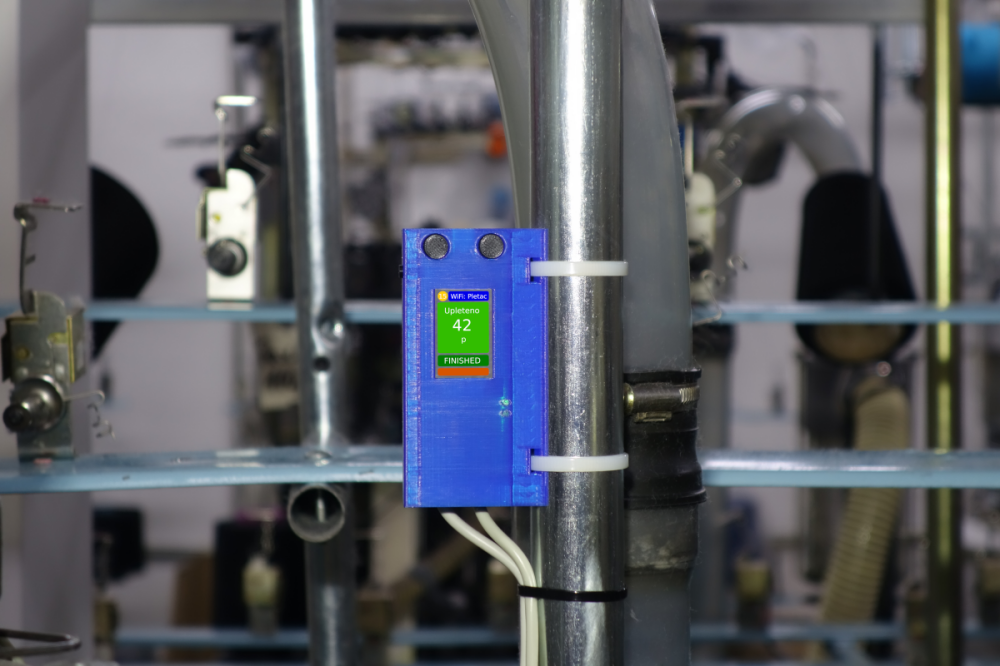
\includegraphics[width=\textwidth]{img/V2-uchyceni.png}
    \caption{Senzor na stroji}
    \label{fig:SenzorNaStroji}
\end{figure}


\newpage
